\documentclass[10pt, aspectratio=169]{beamer} % 16:9 宽屏, 10pt

% 1. 设置全局使用衬线字体
\usefonttheme{serif}

% 2. 引入必要的宏包
\usepackage{xcolor}
\usepackage{graphicx}
\usepackage{slashed}
\usepackage[skins]{tcolorbox}
\usepackage{ragged2e}
% ----- 必须引入的宏包 -----
\usepackage{booktabs}   % 提供 \toprule, \midrule, \bottomrule (三线表格式)
\usepackage{amsmath}    % 数学公式基础
\usepackage{amssymb}    % 提供 \mathbb{I} 空心大写 I 符号
\usepackage{multirow}   % 处理跨行单元格
\usepackage{bigdelim}   % 核心：用于绘制跨行的大括号 \rdelim

\usepackage{phstyle}

% 强制接管所有 itemize 的正文字体，锁定为绝对大小 8pt，行距 10pt
\setbeamerfont{itemize/enumerate body}{size=\fontsize{8pt}{10pt}\selectfont}

% 如果您连子列表 (第二级、第三级) 也要强制锁死，加上这两行：
\setbeamerfont{itemize/enumerate subbody}{size=\fontsize{7pt}{9pt}\selectfont}
\setbeamerfont{itemize/enumerate subsubbody}{size=\fontsize{6pt}{8pt}\selectfont}

\begin{document}

% ==============================================================================
% Slide 1: Title Page (标题页)
% ==============================================================================
\begin{frame}
\mysubtitle{}
\vspace*{\fill}
\mytitle{Analysis of Symmetry of 2-point Correlation Functions in Finite Temperature QCD}
\centering{Using Möbius Domain-Wall Fermions}
\vspace{1cm}

\centering{
\mytext{Junxiong Nie, U. Osaka}
\mytext{for JLQCD Collaboration}
}
\vspace*{\fill}
\end{frame}

% ==============================================================================
% Slide 2: Outline (大纲页)
% ==============================================================================
\begin{frame}
\myheading{Outline}
\vfill
\begin{center} % 1. 让内部的 minipage 整体居中显示
    \begin{minipage}{0.55\textwidth} % 2. 设定一个占屏幕宽度的 55% 的文本框 (内部默认左对齐)

        \mybullet Research Background \\[0.5em]
        \mybullet Theoretical Background \\[0.5em]
        \mybullet Lattice Simulation Setup \\[0.5em]
        \mybullet Numerical Results \\[0.5em]
        \mybullet Summary and Outlook

    \end{minipage}
\end{center}
\vfill
\end{frame}


% ==============================================================================
% Slide 4: Research Background (研究背景)
% ==============================================================================
\begin{frame}
\myheading{Research Background}
\setbeamerfont{itemize/enumerate body}{size=\fontsize{11pt}{14pt}\selectfont}
\fontsize{11pt}{14pt}\selectfont
\vfill
\begin{itemize}
%According to {\scriptsize [Pisarski \& Wilczek (1983)]},
\item The behavior of $U(1)_{\rm A}$ axial symmetry restoration is important to
the order of the chiral phase transition (and universality class if it is 2nd-order), so as our prediction capability with perturbative method
\item The historical effective linear sigma model analysis showed the $U(1)_{\rm A}$ can not be restored before the transition, if the transition is second order, due to the non-existence of stable IR fixed point under non vanish anomalus $U(1)_{\rm A}$ effect in 2 flavor case
\item Previous Lattice simulation study, such as HotQCD, concluded that the chiral phase transition is second order and extracted the universal coefficient, while $U(1)_{\rm A}$ is restored near 1.5$T_c \sim 2 T_c$
\end{itemize}
\vfill
\end{frame}

\begin{frame}
\myheading{Motivation for this work}
\setbeamerfont{itemize/enumerate body}{size=\fontsize{11pt}{14pt}\selectfont}
\fontsize{11pt}{14pt}\selectfont
\begin{itemize}
\item However, the higher loop linear sigma model study and Functional Renormalization Group analysis showed there's nontrivial stable IR fixed point and also the possibility of weak 1st order transition. So, the observation of universal behavior is not enough to conclude the $U(1)_{\rm A}$ symmetry behavior and also the universality class
\item The previous study use Highly Improved Staggered fermion that breaks the chiral symmetry behavior in finite lattice spacing non-negligbly. So these previous conclusions of $U(1)_{\rm A}$ restoration need to be careful re-examined
\item The previous work in the 2-flavor case by JLQCD
 {\scriptsize [Phys. Rev. D \textbf{111}, 114506 (2025)]}
using the  Möbius Domain-Wall fermions  is consistent
with the scenario that
 both  $SU(2)_L \times SU(2)_R$ chiral symmetry and $U(1)_{\rm A}$ symmetry are effectively restored near $T_c \approx 165(3)$ MeV.

\item  We extend this investigation to the more realistic $N_f=2+1$ QCD adding strange quark
\item  We examine the symmetry breaking by mesons screening masses\end{itemize}
\vfill
\end{frame}

\begin{frame}
\myheading{Main part of this work}
\setbeamerfont{itemize/enumerate body}{size=\fontsize{11pt}{14pt}\selectfont}
\fontsize{11pt}{14pt}\selectfont
\begin{itemize}
\item  We extend this investigation to a more realistic $N_f=2+1$ QCD case adding strange quark
\item  We improve it to finer lattice size up to $L48^3\times T16$
\item  We measured spatial two point correlation function data and analysed the symmetry restoration behavior for physical point with different beta and chiral limit case by a fixed beta case with varying quark masses and lattice size
\item  We examine the symmetry breaking by mesons screening masses as a more phenomenologically effective observable followed the idea of work in the 2-flavor case by JLQCD
 {\scriptsize [Phys. Rev. D \textbf{111}, 114506 (2025)]} \end{itemize}
\vfill
\end{frame}
%, to determine if $U(1)_{\rm A}$ restoration persists near the physical point.
% ==============================================================================
% Slide 4: Symmetry of QCD (QCD的对称性)
% ==============================================================================
\begin{frame}
\myheading{Symmetry of QCD}
\vfill
QCD: \hfill
 $\mathcal{Z} =
\int \mathcal{D} A \mathcal{D}\bar{q} \mathcal{D}qe^{-
S}$, Gauge Boson+Fermion\hfill\null

\vspace{1em}
$S =
\int d^4x \left[ - \frac{1}{4} \mathrm{Tr} F \wedge \star F
+ \bar q_a (i \slashed{D} - m_a) q_a \right]$, $a$ in
[1,$N_f$]

\vspace{1em}
Specifically,in the up-down quark mass zero limit:

Flavored chiral symmetry $SU(2)_L \times SU(2)_R$ :
\[
    q \to \exp(i\alpha_a T^a + i\beta_a T^a \gamma_5)q, \quad \bar{q} \to \bar{q} \exp(-i\alpha_a T^a + i\beta_a T^a \gamma_5),
\]

$U(1)_A$ Symmetry :
\[
    q \to \exp(i\epsilon\gamma_5)q, \quad \bar{q} \to \bar{q} \exp(i\epsilon\gamma_5),
\]

We use the mass difference of the screening masses of different channels to
estimate the degree of the symmetry breaking.
\vfill
\end{frame}

% ==============================================================================
% Slide 5: Meson Correlation Functions (介子关联函数)
% ==============================================================================
\begin{frame}
\myheading{ Meson Correlation Functions}
\vfill
We consider the
following set of meson operators
\begin{gather*}
    O_\Gamma(x) = \bar{q}(x)\Gamma F^aq(x), \\[2ex]
    \Gamma \in \left\{ \mathbf{1}(S), \gamma_5(P), \gamma_\mu(V), \gamma_\mu\gamma_5(A), \sigma_{\mu\nu} = \frac{i}{2}[\gamma_\mu, \gamma_\nu](T), \sigma_{\mu\nu}\gamma_5(X) \right\}
\end{gather*}

And we measure the two-points correlation function of the meson operators of different channels.
Accroding to the symmetry properties, the asymptotic behavior of the 2-point correlation function at large distances should be approximately be $a \rm{Cosh}(m_\Gamma(x-L/2)) $
\vfill
\end{frame}




% ==============================================================================
% Slide 6: Symmetry of Correlation Functions (关联函数的对称性与算符配对)
% ==============================================================================
\begin{frame}
\myheading{Symmetry of Correlation Functions}

% --- 变换定义 ---
\begin{itemize}
    \item Flavored chiral symmetry $SU(2)_L \times SU(2)_R$ :
    {\small\hfill
    \( \delta_C O_\Gamma^a = \frac{i}{2} \beta_b \bar{q} \left( \{\Gamma, \gamma_5\} \frac{1}{2} \delta^{ab} \mathbf{1} + [\Gamma, \gamma_5] i \epsilon^{bac} \frac{\tau^c}{2} \right) q \)}
    \hfill\null

    \item $U(1)_A$ Symmetry :
    {\small\hfill
    \( \delta_A O_\Gamma^a = i \epsilon \bar{q} \{\Gamma, \gamma_5\} \frac{\tau^a}{2} q \)}
    \hfill\null
\end{itemize}


% --- 对照表与配对关系 ---
\begin{columns}[T]
    % 左侧：算符变换对照表
    \column{0.3\textwidth}
    \centering
    \vspace{8pt}
    \small
    \renewcommand{\arraystretch}{1.2}
    \begin{tabular}{|c|c|c|}
        \hline
        $\Gamma$ & $[\Gamma, \gamma_5]$ & $\{\Gamma, \gamma_5\}$ \\ \hline
        $\mathbf{1} (S)$ & & $\gamma_5$ \\ \hline
        $\gamma_5 (P)$ & & $\mathbf{1}$ \\ \hline
        $\gamma_\mu (V)$ & $\gamma_\mu \gamma_5$ & \\ \hline
        $\gamma_\mu \gamma_5 (A)$ & $\gamma_\mu$ & \\ \hline
        $\sigma_{\mu\nu} (T)$ & & $\sigma_{\mu\nu} \gamma_5$ \\ \hline
        $\sigma_{\mu\nu} \gamma_5 (X)$ & & $\sigma_{\mu\nu}$ \\ \hline
    \end{tabular}

    % 右侧：对称性配对及结论
    \column{0.7\textwidth}
    \vspace{8pt}
    \centering
    \footnotesize
    \renewcommand{\arraystretch}{1.2}
    \setlength{\tabcolsep}{3pt}
% 表格列设计：共5列。前3列为数据，第4列处理第一层括号，第5列处理最外层括号
    \begin{tabular}{ccc @{\hspace{2pt}}ll}
        \toprule
        $\Gamma$ & Reference Name & Abbr. & \multicolumn{2}{l}{Symmetry Correspondences} \\
        \midrule

        $\mathbb{I}$ & Scalar & S & \rdelim\}{2}{*}[ \scriptsize{$\ U(1)_A$} ] & \\
        $\gamma_5$ & Pseudo Scalar & PS & & \\ % 注：原图拼写就是 Psuedo，此处照抄原图

        $\gamma_1, \gamma_2$ & Vector & $V$ & \rdelim\}{2}{*}[ \footnotesize{$\ SU(2)_L \times SU(2)_R$} ] & \hspace{-1.5em}\rdelim\}{4}{*}[ \footnotesize{$\ SU(2)_{CS}$} ] \\
        $\gamma_1\gamma_5, \gamma_2\gamma_5$ & Axial Vector & $A$ & & \\

        $\gamma_4\gamma_3$ & Tensor & $T_t$ & \rdelim\}{2}{*}[ \footnotesize{$\ U(1)_A$} ] & \\
        $\gamma_4\gamma_3\gamma_5$ & Axial Tensor & $X_t$ & & \\

        \bottomrule
    \end{tabular}

\end{columns}

\end{frame}

% ==============================================================================
% Slide 7: Order of Chiral Phase Transition (手征相变的阶)
% ==============================================================================
\begin{frame}
\myheading{Order of Chiral Phase Transition}
\setbeamerfont{itemize/enumerate body}{size=\fontsize{11pt}{14pt}\selectfont}
\fontsize{11pt}{14pt}\selectfont
\vfill
\begin{itemize}
    \item Perturbative $4-\epsilon$ expansion Renormalization Group Analysis of effective linear sigma model for $\langle \bar{q} P_L q \rangle$. They found for $N_f > \sqrt{3}$ flavor symmetry, there's no stable IR fixed point. {\scriptsize [Pisarski-Wilczek (1983)]} \\
    \item The anomaly effect term is a determinant term in the effective linear sigma model, which is a $N_f$-th order term. For $N_f \geq 3 $ flavor case, it doesn't change the order of the transition.  \\
   \item But for $N_f = 2$ flavor case, it becomes a quadratic term, which can smooth out the singularity and change the transition to second order. If the anomaly effect still exists, the transition can be $\mathrm{O}(4)$ class. If the anomaly effect is  suppressed and  $\mathrm{U}(1)_{\mathrm{A}} $ symmetry is restored before or at the critical temperature $T_c$, then transition should be still first order
\item But recently higher-loop computations and FRG computations suggested different possibilities {\scriptsize [E.Vicari ,F.Basile, A.Pelissetto 2005 , G. Fejos 2022]}, and Conformal Boostrap results indicate some interesting points too{\scriptsize [Nakayama Ohtsuki 2016}
\end{itemize}
\vfill
\end{frame}



% ==============================================================================
% Slide 8: Possible Emergent Larger Symmetry (可能涌现的更大对称性 - 手征自旋对称性)
% ==============================================================================
\begin{frame}
\myheading{Possible Emergent Larger Symmetry}
\setbeamerfont{itemize/enumerate body}{size=\fontsize{10pt}{12pt}\selectfont}
\fontsize{10pt}{12pt}\selectfont
\vfill

\begin{itemize}
\item Perturbative analysis of screening masses from NRQCD$_3$
{\scriptsize{[Laine, M., Vepsäläinen, M. (2004)]}}:  $\left[ 2 M - \frac{\nabla_{\ensuremath{\boldsymbol{r}}}^2}{\pi T} +
\right. $ $ \left. V(\ensuremath{\boldsymbol{r}}) \right]\Psi_0 =
m_{\ensuremath{\operatorname{scr}}} \Psi_0$, where $M$ is the mass parameter in model
\item
$M = \pi T + g^2 T \frac{C_F}{8 \pi} +\mathcal{O} (g^4 T)$

\item We write $(m_{src}- 2M)$ as $g_{\mathrm{E}}^2  \frac{C_F}{2 \pi} \hat E_0$, where $\hat E_0$(around 0.38237 for 2-flavor) is computed numerically

\item For two falvor case, we got $m_{\mathrm{scr}}= 2\pi T +
 g_{\mathrm{E}}^2  \frac{C_F}{2 \pi} (1/2+\hat E_0 )= 2\pi T
+ 0.1872g^2 T
$

\item It  predicts the flavor non-singlet channel will tend to behave same screening mass.
Thus,a larger symmetry, Chiral-Spin Symmetry $SU(2)_{CS}$ , may emerge\begin{align*}
    q &\to \exp(i\Sigma^i\epsilon_i)q, \\
    \bar{q} &\to \bar{q}\gamma_0 \exp(-i\Sigma^i\epsilon_i)\gamma_0,
\end{align*}

where $\Sigma^i$ has three components,

\[
    \Sigma^i = (\gamma_k, -i\gamma_5\gamma_k, \gamma_5), \quad k = 1, 2.
\]

\end{itemize}
\vfill
\end{frame}

% ==============================================================================
% Slide 9: Lattice QCD Setup - Residual Mass (晶格QCD数值设置 - 残余质量表)
% ==============================================================================
\begin{frame}
\myheading{Lattice QCD Numerical Setup}
\vfill
\mybullet Möbius Domain-Wall Fermions:
The effective 4D operator is[Brower, R. C., Neff, H., \& Orginos, K.~(2012)]:
\[ {\color{black}{D^{\text{4D}}_{\ensuremath{\operatorname{DW}}} (m) = \frac{1
   + m}{2} + \frac{1 - m}{2} \gamma_5 \tanh (L_s \tanh^{- 1} (H_M)),}} \]
where {\color{black}{$m$}} is the bare quark mass, and the Möbius kernel
{\color{black}{${\color{black}{H_M}}$}} is $ {\color{black}{H_M = \gamma_5  \frac{2 D_W}{2 + D_W}}} $

\vspace{1em}
The precision of chiral symmetry could be estimated by Residual Mass $m_{res}$, and at low beta case is not so good:

\begin{table}[htbp]
    \centering
    \scriptsize
    \begin{tabular}{lcccccccc}
        \toprule
        $T$ (MeV) & 138 & 145 & 153 & 157 & 164.5 & 176 & 202 & 241.6 \\
        \midrule
        $m_{res}/m_l$ & 0.9087 & 0.5360 & 0.3394 & 0.2744 & 0.1836 & 0.1041 & 0.0299 & 0.0049 \\
        $m_{res}$ & 7.31e-4 & 4.98e-4 & 3.40e-4 & 2.80e-4 & 1.91e-4 & 1.08e-4 & 2.81e-5 & 3.75e-6 \\
        \bottomrule
    \end{tabular}
\end{table}
\vfill
\end{frame}

% ==============================================================================
% Slide 10: Lattice QCD Setup - Simulation Table (晶格QCD数值设置 - 参数与温度表)
% ==============================================================================
\begin{frame}
\myheading{Lattice QCD Numerical Setup}
\vfill
The simulation is run with lattice size $48^3 \times 16$ (near the physical point):

\vspace{1ex} % 增加一点文字与表格的间距

\begin{table}[htbp]
    \centering
    \renewcommand{\arraystretch}{1.2} % 稍微拉大行距，看起来更舒适
    \begin{tabular}{cccc}
        \toprule
        $\beta$ & $T$ (MeV) & $am_s$ & $am$ \\
        \midrule
        4.13 & 138 & 0.043547 & 0.000805 \\
        4.15 & 145 & 0.040843 & 0.000930 \\
        4.17 & 153 & 0.038400 & 0.001001 \\
        4.18 & 157 & 0.037265 & 0.001022 \\
        4.20 & 164.5 & 0.035150 & 0.001041 \\
        4.23 & 176 & 0.032315 & 0.001033 \\
        4.30 & 202 & 0.026930 & 0.000939 \\
        \bottomrule
    \end{tabular}
\vfill
\end{table}

\end{frame}

% ==========================================
% 下面是重新排版的带有 PDF 图片的幻灯片
% ==========================================

% ==============================================================================
% Slide 11: Lattice Measurements & Configurations (格点测量与配置数)
% ==============================================================================
\begin{frame}
\myheading{Lattice Measurements \& Configurations}
\vfill
\setbeamerfont{itemize/enumerate body}{size=\fontsize{9pt}{12pt}\selectfont}
\begin{itemize}
    \item We performed measurements for each beta parameters, each channels, and each directions
    \item To  improve the quality of data, we performed \textbf{16-source} measurements
    \item The total number of configurations ($N_{\mathrm{conf}}$) analyzed for each temperature/$\beta$ are counted below :
\end{itemize}

\vspace{1em}

\begin{table}[htbp]
    \centering
    \scriptsize
    \renewcommand{\arraystretch}{1.25}
    \begin{tabular}{lccccccc}
        \toprule
        $\beta$ & 4.13 & 4.15 & 4.17 & 4.18 & 4.20 & 4.23 & 4.30 \\
        \midrule
        $T$ (MeV) & 138 & 145 & 153 & 157 & 164.5 & 176 & 202 \\
        No. of Confs ($N_{\mathrm{conf}}$) & 395 & 398 & 396 & 402 & 407 & 395 & 404 \\
        Total Meas. ($16 \times N_{\mathrm{conf}}$) & 6320 & 6368 & 6336 & 6432 & 6512 & 6320 & 6464 \\
        \bottomrule
    \end{tabular}
\end{table}
\vfill
\end{frame}

% ==============================================================================
% Slide 12: Meson Channels & Directional Averaging (介子信道与方向平均)
% ==============================================================================
\begin{frame}
\myheading{Meson Channels \& Directional Averaging}
\vfill
\setbeamerfont{itemize/enumerate body}{size=\fontsize{9pt}{12pt}\selectfont}
\begin{itemize}
    \item To improve the data quality, the correlation functions of each meson channel are averaged over all equivalent spatial directions and components.
    \item The directional averaging components is summarized below:
\end{itemize}

\vspace{0.5em}

\begin{table}[htbp]
    \centering
    \scriptsize
    \renewcommand{\arraystretch}{1.25}
    \begin{tabular}{lccl}
        \toprule
        Channel & Components & Averaged Directions (configured in \texttt{config.py}) \\
        \midrule
        \textbf{AV} (Axial Vector) & 6 & $X$ (\texttt{AVector2}, \texttt{AVector3}), $Y$ (\texttt{AVector1}, \texttt{AVector3}), $Z$ (\texttt{AVector1}, \texttt{AVector2}) \\
        \textbf{Vec} (Vector) & 6 & $X$ (\texttt{Vector2}, \texttt{Vector3}), $Y$ (\texttt{Vector1}, \texttt{Vector3}), $Z$ (\texttt{Vector1}, \texttt{Vector2}) \\
        \textbf{S} (Scalar) & 3 & $X, Y, Z$ (\texttt{TVector4}) \\
        \textbf{PS} (Pseudo-Scalar) & 3 & $X, Y, Z$ (\texttt{TAVector4}) \\
        \textbf{Tt} (Tensor) & 3 & $X$ (\texttt{TVector1}), $Y$ (\texttt{TVector2}), $Z$ (\texttt{TVector3}) \\
        \textbf{Xt} (Axial Tensor) & 3 & $X$ (\texttt{TAVector1}), $Y$ (\texttt{TAVector2}), $Z$ (\texttt{TAVector3}) \\
        \bottomrule
    \end{tabular}
\end{table}
\vfill
\end{frame}

% ==============================================================================
% Slide 13: Extracting Screening Masses: Methodology (抽取筛选质量：方法学)
% ==============================================================================
\begin{frame}
\myheading{Extracting Screening Masses: Methodology}
\vfill
\setbeamerfont{itemize/enumerate body}{size=\fontsize{9.5pt}{13pt}\selectfont}
\begin{itemize}
    \item We fit the ratio of averaged correlation functions to the analytic form:
    \[
        \frac{C(x)}{C(x + 1)} = \frac{\cosh(m(x - L/2))}{\cosh(m(x + 1 - L/2))}
    \]
    to extract the effective mass $m(x)$ at each spatial coordinate $x$.

    \item \textbf{Jackknife Method}: Used to calculate unbiased statistical errors of the fitted masses and eliminate autocorrelation bias in HMC trajectories.

    \item \textbf{Binning Analysis}: Performed to ensure the Jackknife error estimate reaches saturation and accurately reflects the statistical uncertainty.

    \item \textbf{Screening Mass Extraction}: The physical screening mass $m_{\text{scr}}$ is obtained by identifying the long-distance plateau of the effective mass $m(x)$.
\end{itemize}
\vfill
\end{frame}

% ==============================================================================
% Slide 14: Extracting Screening Masses: Fit Examples (抽取筛选质量：拟合示例)
% ==============================================================================
\begin{frame}
\myheading{Extracting Screening Masses: Fit Examples}
\vfill
\begin{columns}[T]
    % 左侧图: Correlation data
    \begin{column}{0.48\textwidth}
        \centering
        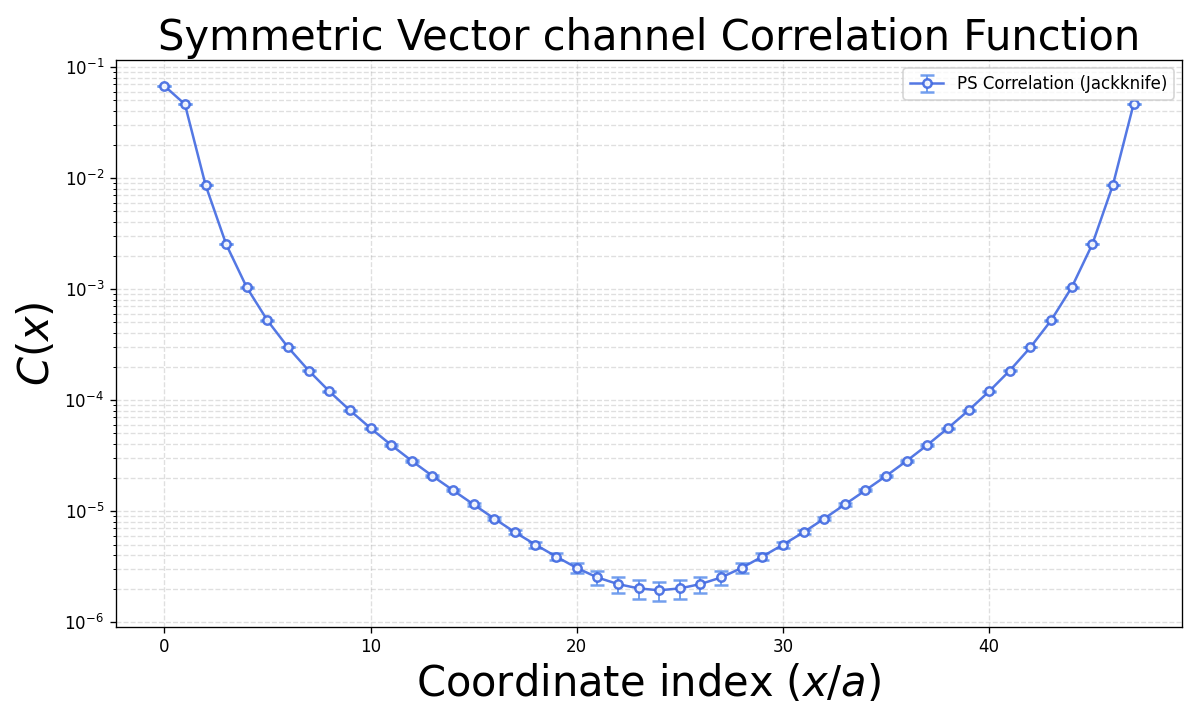
\includegraphics[width=\textwidth]{diff_clean_ps_plot.png}\\
        \vspace{0.2cm}
        {\footnotesize correlation data of Vec channel for $\beta=4.15$(T=153MeV)}
    \end{column}

    % 右侧图: Effective mass
    \begin{column}{0.48\textwidth}
        \centering
        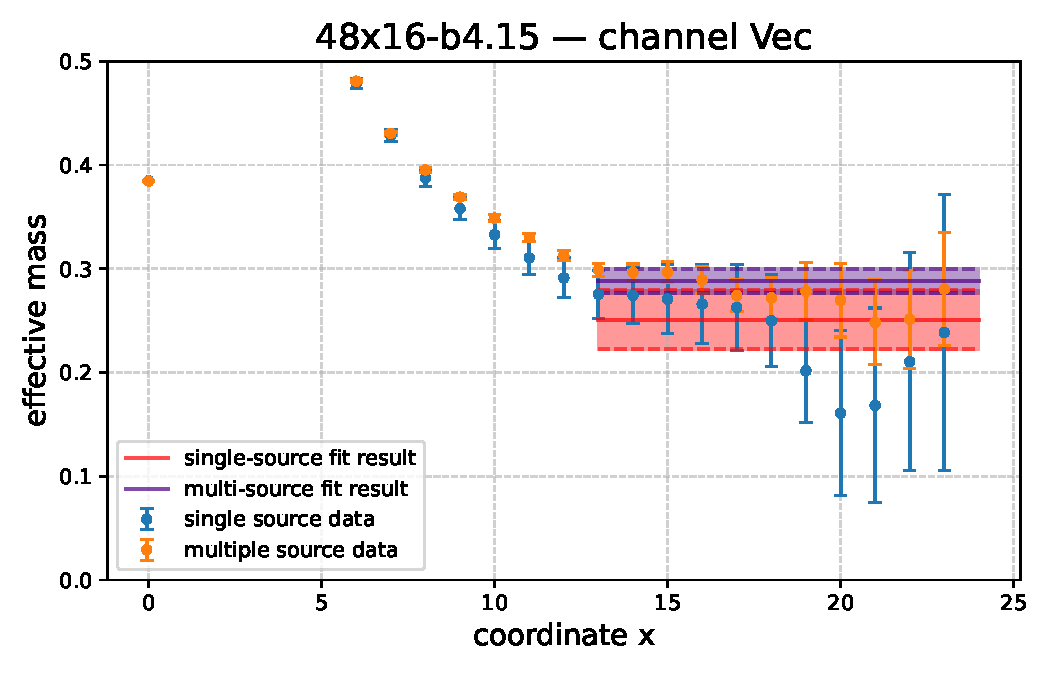
\includegraphics[width=\textwidth]{ratioVec.pdf}\\
        \vspace{0.2cm}
        {\footnotesize effective mass of Vec channel for $\beta=4.15$(T=153MeV)}
    \end{column}
\end{columns}
\vfill
\end{frame}



% ==============================================================================
% Slide 12: Numerical Results (数值结果 - 筛选质量与对称性破缺对比图)
% ==============================================================================
\begin{frame}
\myheading{Numerical Results}
\vfill
Multi-source analysis results(I draw also $T_c$ =165(3) MeV range as the grey band){\scriptsize [Y. Aoki, D. Ward et al., Phys. Rev. D \textbf{111}, 114506 (2025)]}:
\begin{columns}[T] % [T] 表示顶部对齐
    % 左侧图: S vs PS
    \begin{column}{0.48\textwidth}
        \centering
        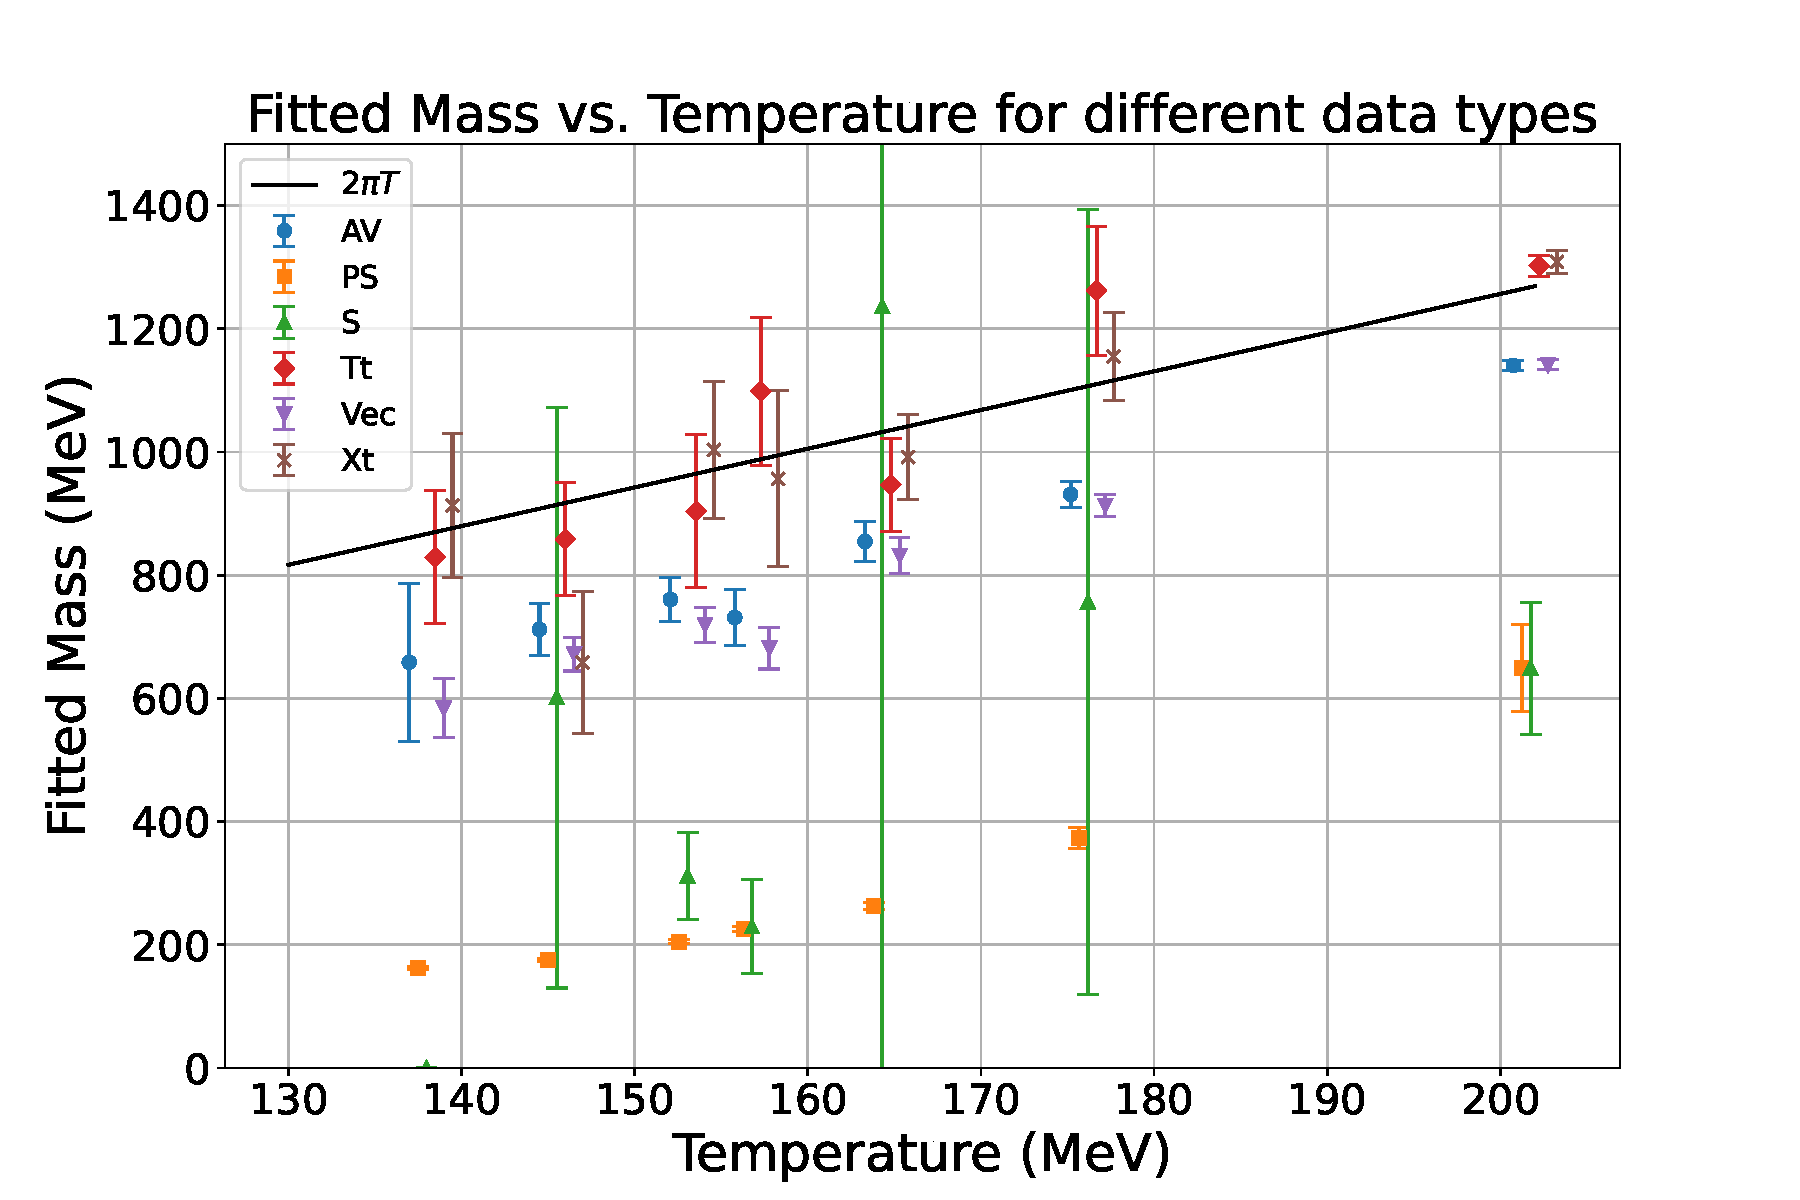
\includegraphics[width=\textwidth]{simulation_results.pdf}\\
        \vspace{0.2cm}
        {\footnotesize simulated effective masses of different channels}
    \end{column}

    % 右侧图: Xt vs Tt
    \begin{column}{0.48\textwidth}
        \centering
        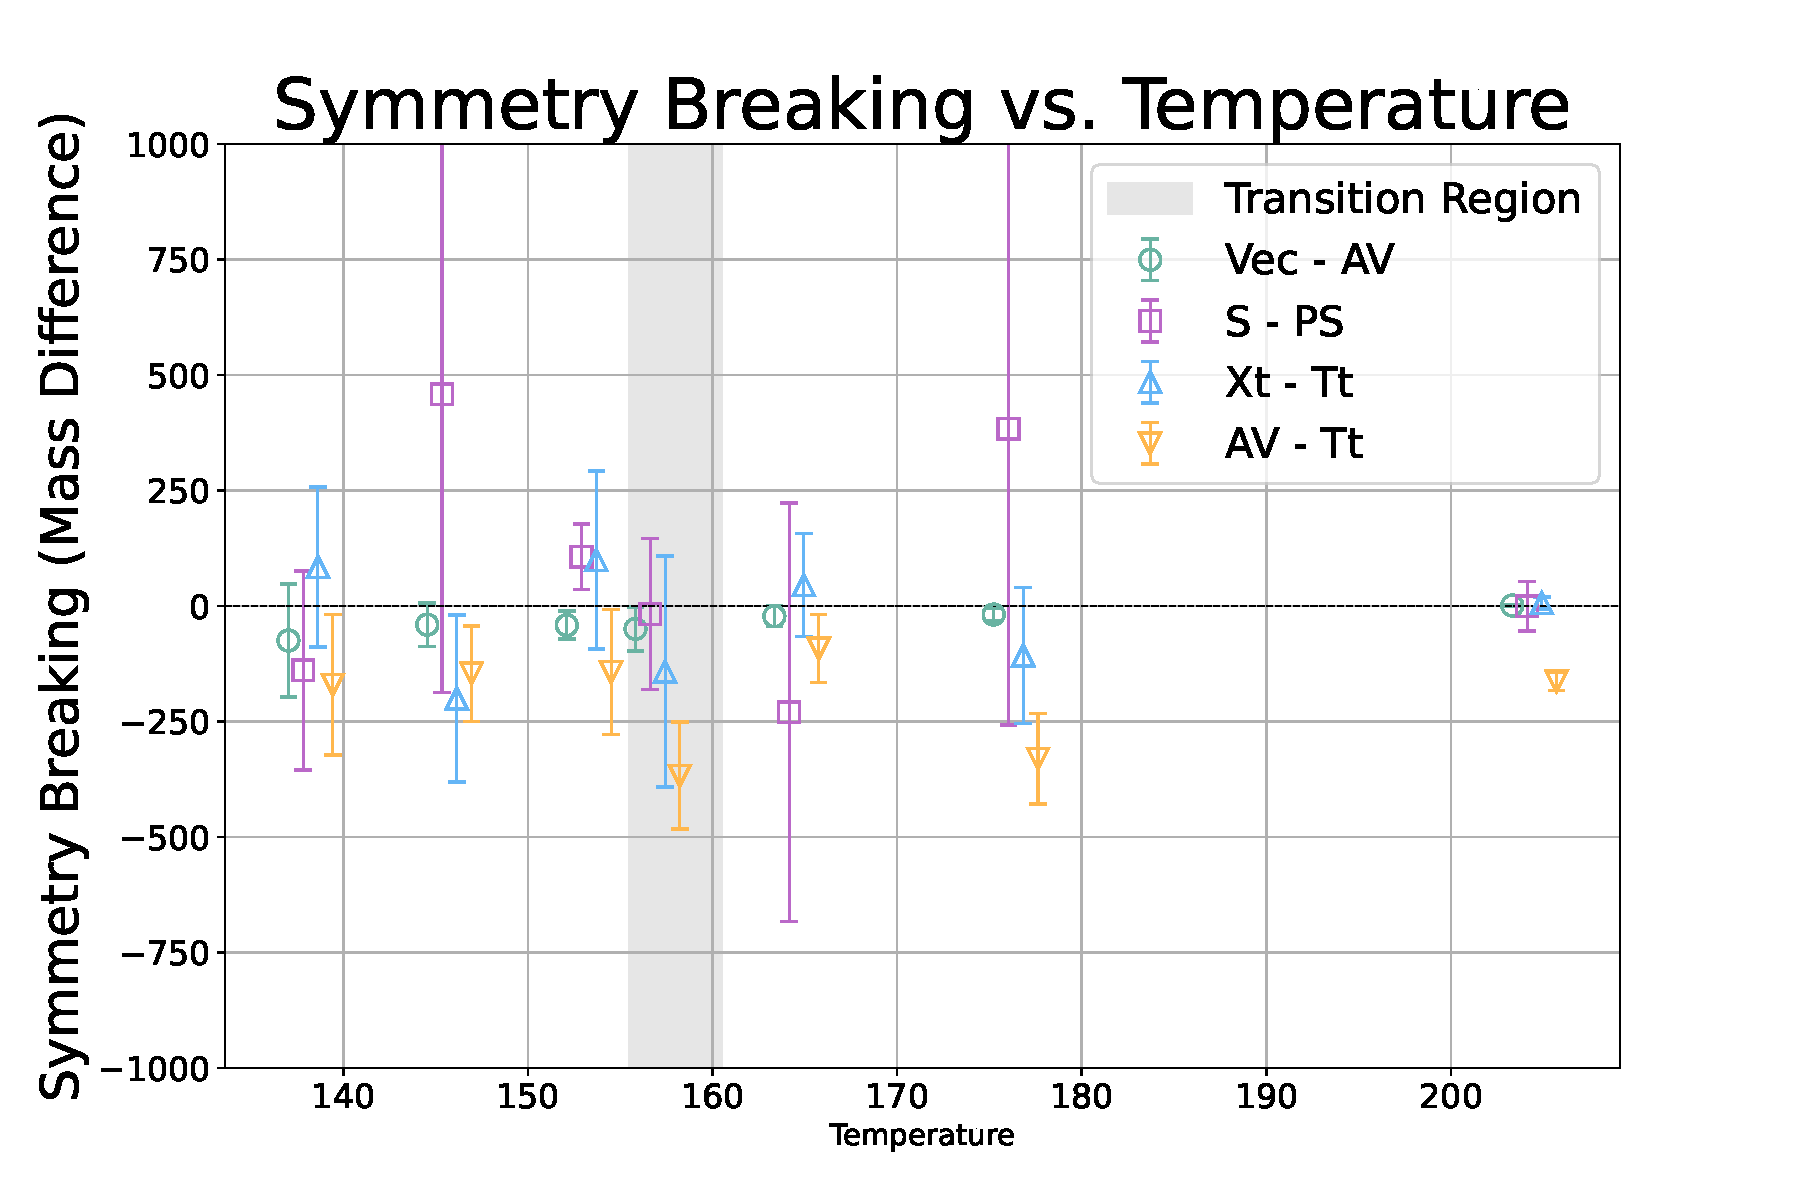
\includegraphics[width=\textwidth]{symmetry_breaking.pdf}\\
        \vspace{0.2cm}
        {\footnotesize Symmetry breaking of different channels}
    \end{column}
\end{columns}

\vfill
\end{frame}


% ==============================================================================
% Slide 13: SU(2)_L x SU(2)_R Chiral Symmetry (手征对称性恢复结果)
% ==============================================================================
\begin{frame}
\myheading{$SU(2)_L \times SU(2)_R$ Chiral Symmetry}
\vfill
\begin{columns}[c] % [c] 表示垂直居中对齐
    % 左边放文字说明 (占屏幕 40% 宽度)
    \begin{column}{0.4\textwidth}
        \justifying
      \mybullet  This indicates the restoration of the $SU(2)_L \times SU(2)_R$ chiral symmetry (e.g., AV vs Vec channels).\\
      \mybullet  At $T=0$, the difference between $a_1$ ($1230$ MeV) and $\rho$ meson ($775$ MeV) is around $455$ MeV.\\
      \mybullet  But the pseudo critical temperature is not very clear (due to finite quark mass) \\
    \end{column}

    % 右边放图 (占屏幕 55% 宽度)
    \begin{column}{0.55\textwidth}
        \centering
        % 插入 SU(2) 对应的图，宽度自适应当前列宽
        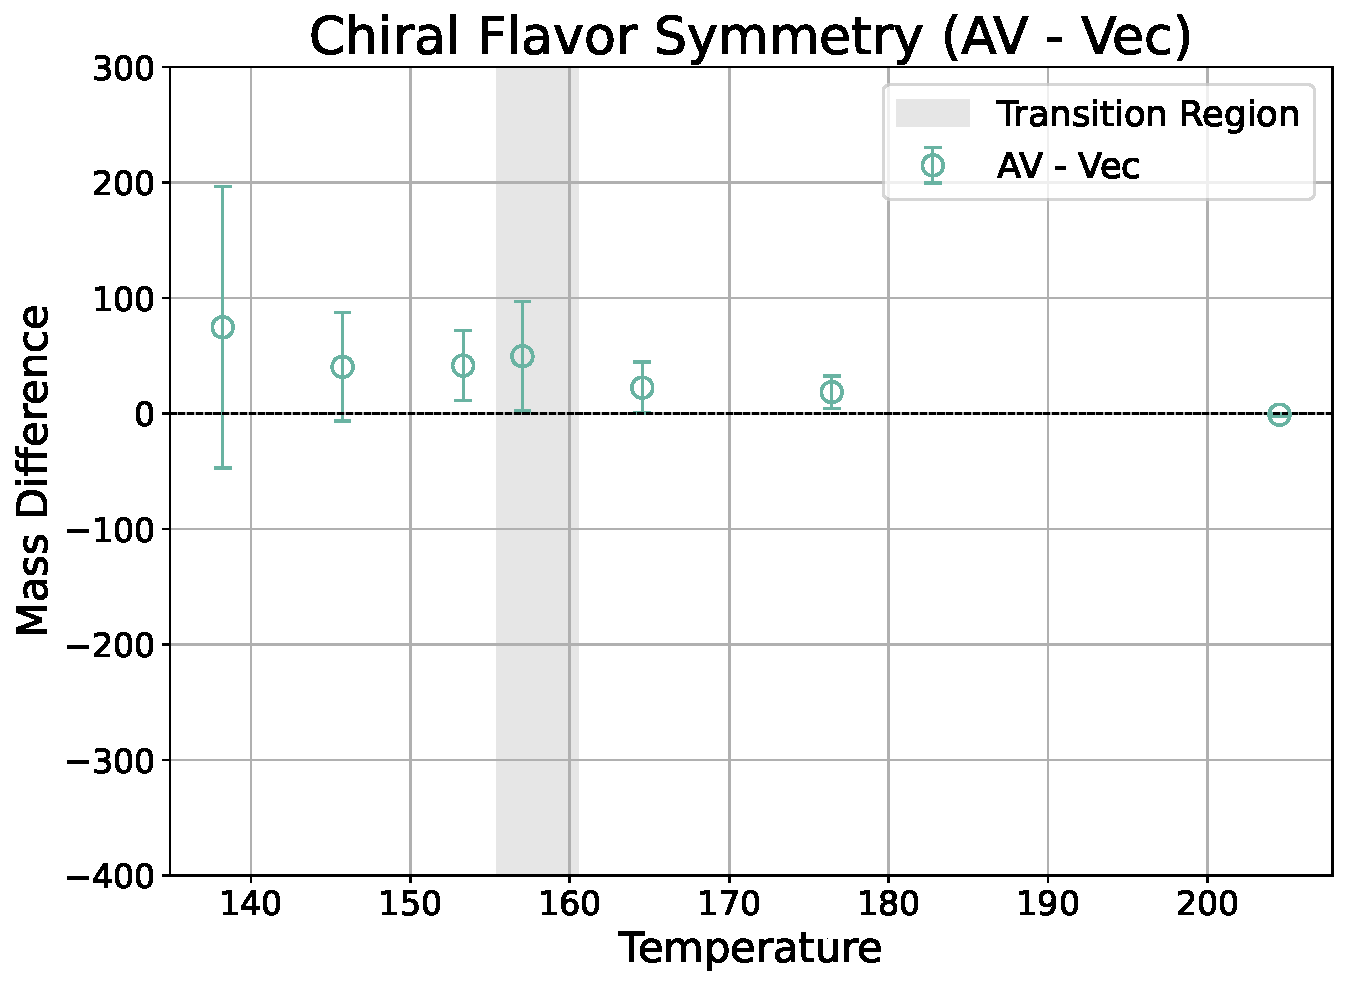
\includegraphics[width=\textwidth]{symmetry_breaking_Chiral_AV_Vec.pdf}
    \end{column}
\end{columns}
\vfill
\end{frame}

% ==============================================================================
% Slide 14: U(1)_A Symmetry (U(1)_A 轴向对称性恢复结果)
% ==============================================================================
\begin{frame}
\myheading{$U(1)_A$ Symmetry}

The difference tends to decrease at high temperatures, suggesting approximate restoration of $U(1)_A$ symmetry (anomaly suppression), compared to the flavour symmetry :

\begin{columns}[T] % [T] 表示顶部对齐
     % 右侧图: Xt vs Tt
    \begin{column}{0.6\textwidth}
        \centering
        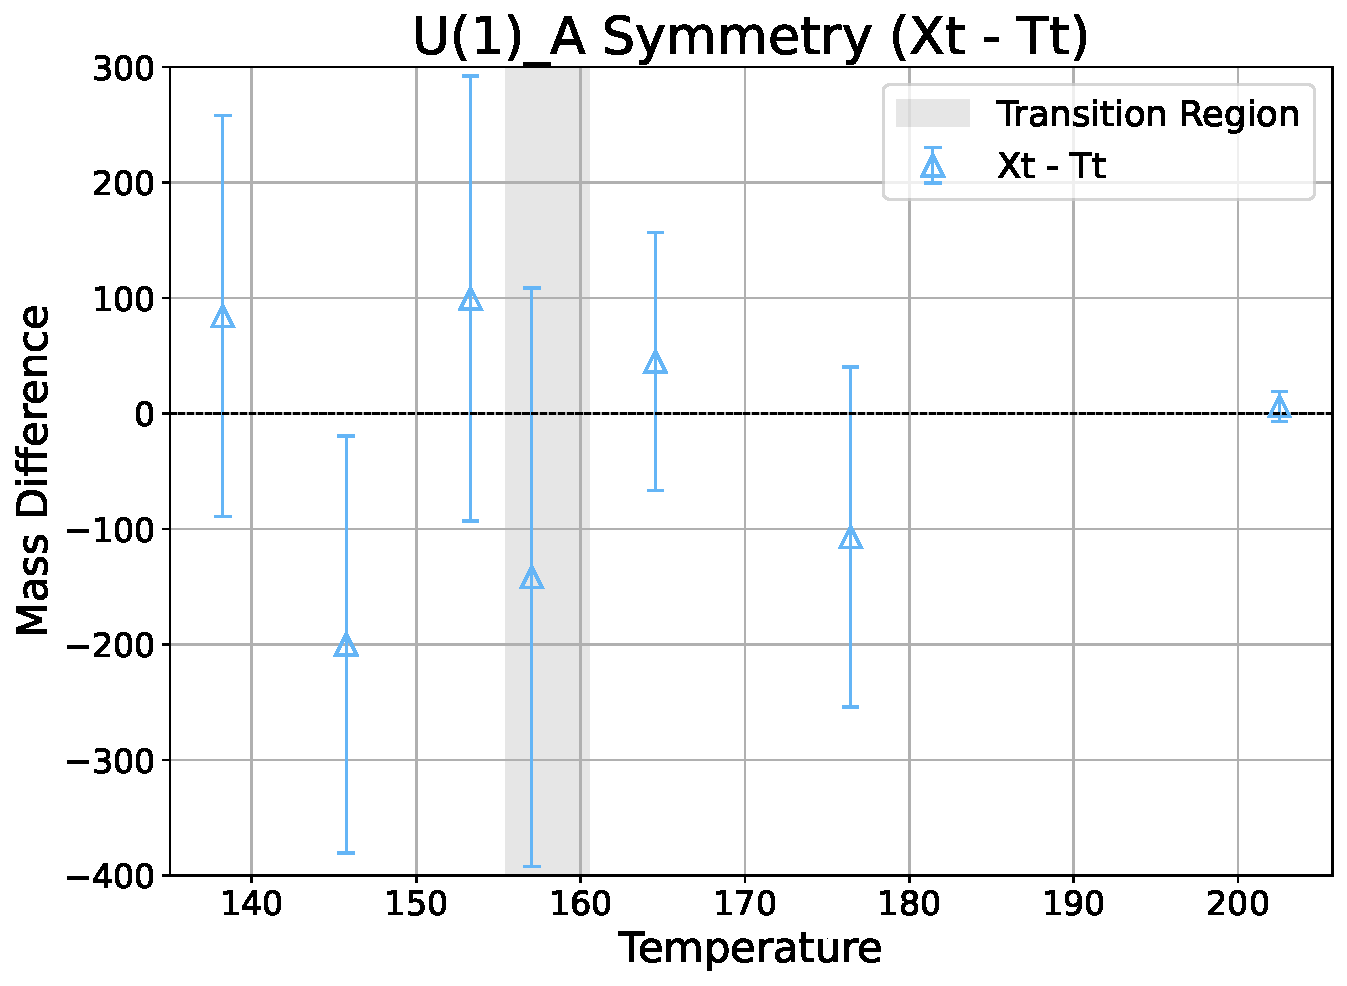
\includegraphics[width=\textwidth]{symmetry_breaking_U1A_Xt_Tt.pdf}\\
        \vspace{0.2cm}
        {\footnotesize Axial Tensor vs Tensor}
    \end{column}

 % 左侧图: S vs PS
    \begin{column}{0.37\textwidth}
        \centering
        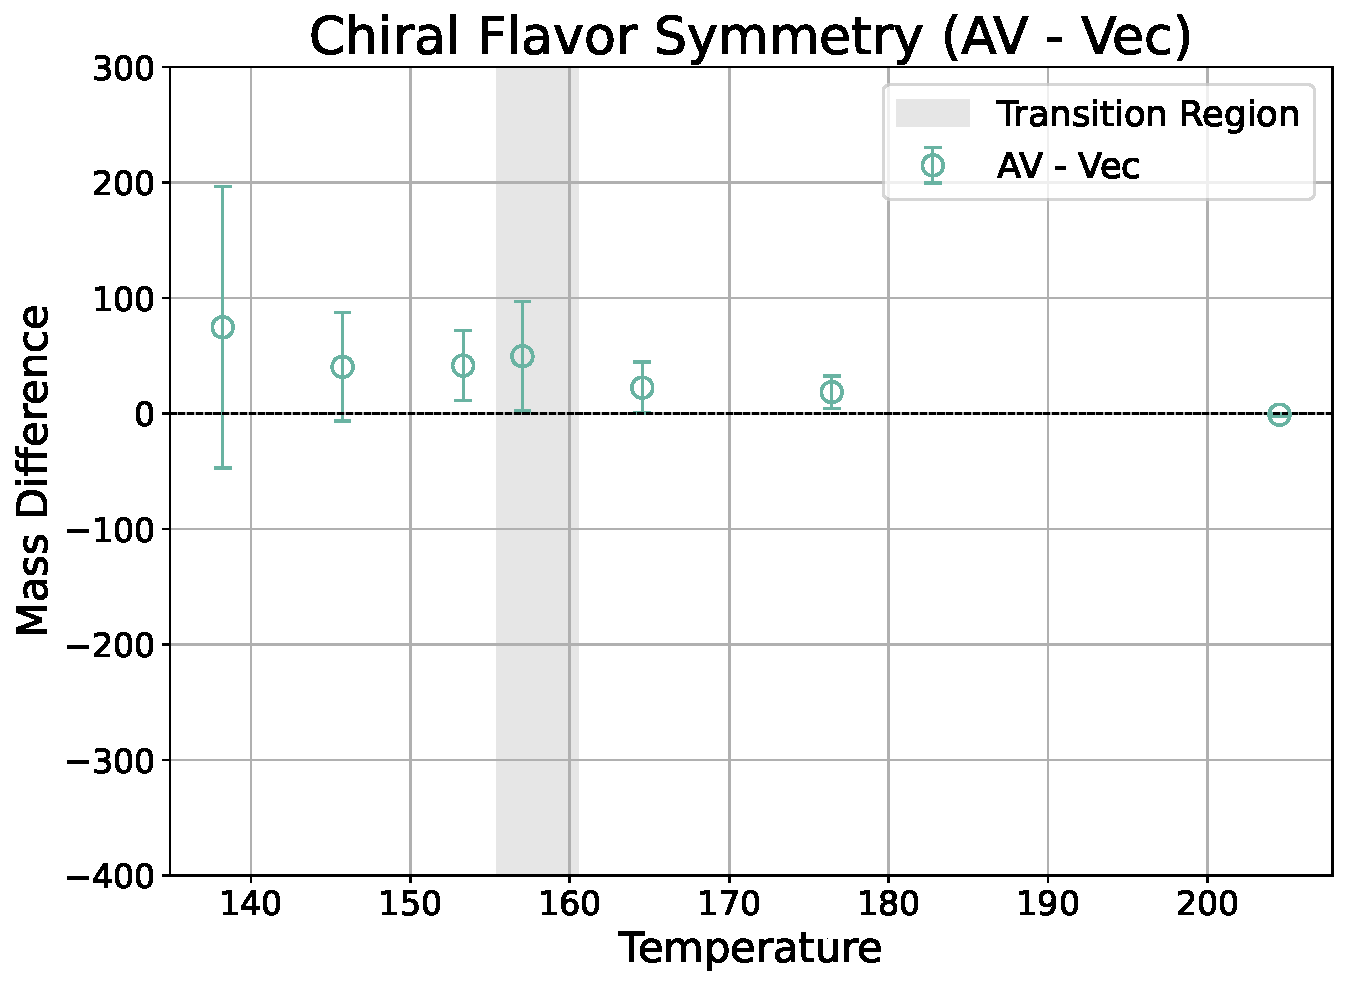
\includegraphics[width=\textwidth]{symmetry_breaking_Chiral_AV_Vec.pdf}\\
        \vspace{0.2cm}
        {\footnotesize Scalar vs Pseudo-Scalar}
    \end{column}

\end{columns}
\end{frame}

% ==============================================================================
% Slide 15: SU(2)_CS Symmetry (手征自旋对称性结果)
% ==============================================================================
\begin{frame}
\myheading{$SU(2)_{CS}$ Symmetry}
\vfill
\begin{columns}[c]
    % 左边放文字
    \begin{column}{0.4\textwidth}
        \justifying
        Observation: Chiral-Spin (CS) symmetry is not yet completely visible at the temperatures analyzed near the phase transition. \\
        \vspace{1em}
        Requires exploration of higher temperature domains.
    \end{column}

    % 右边放图
    \begin{column}{0.55\textwidth}
        \centering
        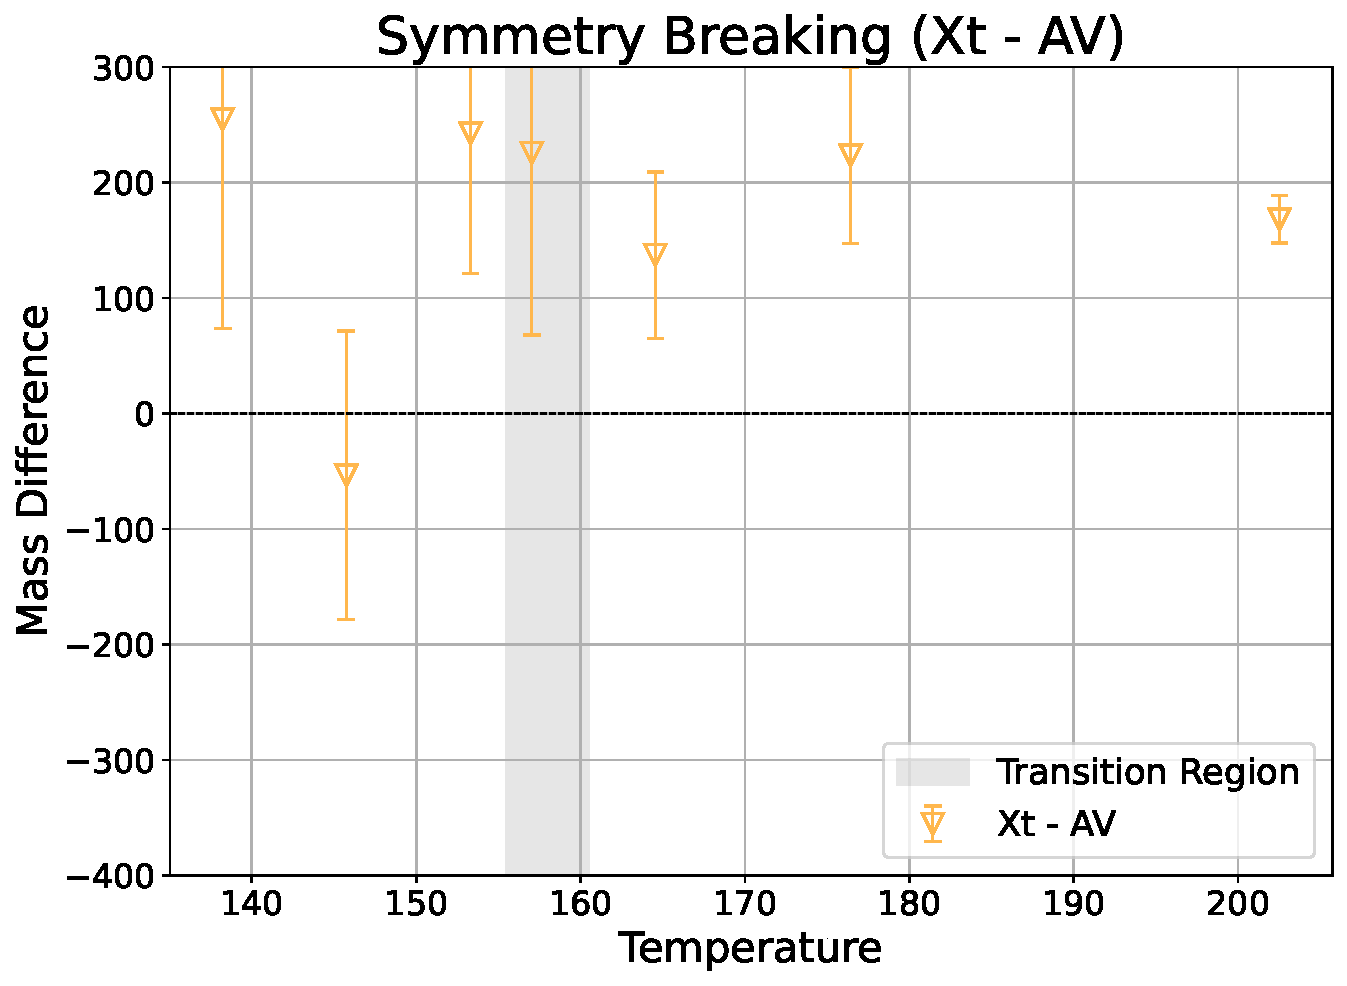
\includegraphics[width=\textwidth]{symmetry_breaking_Xt_AV.pdf}
    \end{column}
\end{columns}
\vfill
\end{frame}

% ==========================================

% ==============================================================================
% Slide 16: Summary and Outlook (总结与展望)
% ==============================================================================
\begin{frame}
\myheading{Summary and Outlook} % 使用您之前定义的标题宏
\setbeamerfont{itemize/enumerate body}{size=\fontsize{11pt}{14pt}\selectfont}
\fontsize{11pt}{14pt}\selectfont
\vfill
% --- 第二部分：Rough Conclusion ---
Summary of the preliminary results:
\vspace{1ex}
\begin{itemize}
    % 默认 itemize 就是实心圆 (bullet)
    \item Focusing on these data, the physical point $N_f=2+1$ QCD does not show clear Chiral Phase Transition behavior as in the chiral limit (which is reasonable).

    \item For $T = 164 \text{ MeV}$, the chiral flavor symmetry and $U(1)_{\mathrm{A}}$ symmetry
breaking are
consistent with zero
 ( but with large errors).

    \item Chiral-Spin symmetry is not visible under T=202MeV.
\end{itemize}

\vspace{1em}
% --- 第一部分：Possible Improvement ---
Possible Improvement:
\vspace{1ex}
\begin{itemize}
    % 使用 \circ 强制将 bullet 改为原图中的空心圆
    \item[\(\circ\)] The data still fluctuated very much, and we want to try to implement more sophisticated statstical method to improve the analysis
    \item[\(\circ\)] We need to determine the critical temperature $T_c$ by chiral susceptibility (also need to improve data quality).
\end{itemize}

\vspace{3ex} % 两部分之间的垂直间距


\vfill
\end{frame}


\end{document}
